\documentclass{article} % For LaTeX2e
\usepackage{nips13submit_e,times}
\usepackage{graphicx}
\usepackage{hyperref}
\usepackage{amsmath}
\usepackage{subcaption}
\usepackage{amssymb}
\usepackage{algorithm}
\usepackage[noend]{algpseudocode}
\usepackage{url}
\usepackage[
abbreviate=false,
backend=biber,
sortcites=true,
sorting=nyt,
sortlocale=en_US,
style=numeric-verb,
maxnames=10
]{biblatex}                     % Bibliography support

\newcommand{\setof}[1]{\ensuremath{\left \{ #1 \right \}}}

\title{Multi-armed Bandits and Reinforcement Learning Approaches to Targeted
Advertising}


\author{
Eric Andrews \\
Seminar: Reinforcement Learning and Its Applications, Spring 2014 \\
Department of Computer Science, University of Helsinki\\\\
}

% The \author macro works with any number of authors. There are two commands
% used to separate the names and addresses of multiple authors: \And and \AND.
%
% Using \And between authors leaves it to \LaTeX{} to determine where to break
% the lines. Using \AND forces a linebreak at that point. So, if \LaTeX{}
% puts 3 of 4 authors names on the first line, and the last on the second
% line, try using \AND instead of \And before the third author name.

\newcommand{\fix}{\marginpar{FIX}}
\newcommand{\new}{\marginpar{NEW}}


\nipsfinalcopy % Uncomment for camera-ready version

\bibliography{sources.bib}
\begin{document}


\maketitle

\begin{abstract}
  TODO
\end{abstract}

\section{Introduction}

In an age where a huge amount of information and news can be found
free-of-charge online, many content producers on the Internet rely on
advertisement revenues to fund their operations. Often this advertisement is
deployed in the form of clickable banner ads, either textual, graphical,
animated or even interactive content, usually separated from the main content,
and designed to attract the interest of visitors. When a visitor clicks such a
banner, they are redirected to the advertiser's site, and the content producer
is financially compensated for the referral.

In this kind of advertising, it is the interest of the content producer to
maximize \emph{click-through rate} (CTR) of the banner ads: the number of times
clicked divided by \emph{impressions}, the number of times shown. If a content
producer has several ad banners it could show to the user, one strategy could
be just to fill up the web site with ads. However this can quickly lead to user
annoyance, and in the worst scenario, cause users to leave the site. Further,
the effectiveness of the advertisements starts to wither as more slots for
banners are introduced, either because a saturation point is hit where users
learn to ignore most of the banners, or there simply isn't room for more
banners on the page.

An alternative strategy is to recognize that there is a limit to the number of
viable banner slots, and attempt to somehow selectively choose the ads to show
according to whom the ad is being displayed to. This is often referred to as
\emph{targeted advertising} or \emph{behavioral targeting}. By adding some
intelligence, we can attempt to show the user advertisements he or she could
potentially be interested in instead of just uniformly picking one out of a
bunch.

% TODO: use of term: targeted advertising vs. behavioral targeting

% TODO: an clump of unsubstantiated claims; find some sources...

% TODO: banner blindness, saturation

This paper introduces two approaches to targeted advertising. First the
simpler, multi-armed bandit model is explored in some detail. It is the classic
example through which the exploration vs.  exploitation trade-off has been
studied. We then delve into some modifications of the model that are useful in
this setting of banner ad selection. After going through this simple model, a
more complex approach called reinforcement learning is considered. This
approach allows us to take into consideration situations in which the agent,
the ad system, can affect the state of the user, e.g. make them annoyed so that
they leave the site.

\section{Related work}

Other approaches to targeted advertising have been explored as well. Chen et
al. \cite{chen2009large} consider a Poisson regression model to predict
click-through rates from user history.  They applied their large-scale
parallelized approach to Yahoo's user base which resulted in great improvement
in CTR.

Work in information retrieval may be applied to targeted advertising as well.
For example personalized news recommendation is in some sense a very similar
problem, albeit from a different viewpoint. \emph{Contextual advertising} is
also concerned with selecting banner ads intelligently, but instead of
targeting the user, the ad is chosen according to the content being served to
the user.

A different but domain-related topic is learning strategies for
\emph{real-time bidding}. Currently web sites can sell ads for banner slots at
an extremely granular level: a single impression. When a user visits a site, a
few hundred millisecond auction is held, in which the advertisers name their
price given the profile of the visiting user. When the time is up, the highest
bidder gets their ad on the site. There have been studies on optimal strategies
for maximizing profits (i.e. balancing ad click-rate and cost) from the
viewpoint of the advertiser with \cite{ding2013multi} and without
\cite{chakraborty2010selective} the multi-armed bandit model. In any case, the
exploration vs exploitation dilemma is highlighted in this setting.

The quite recent field of applying computer science to ad selection goes under
the umbrella term \emph{computational advertising}. Especially software
corporations Microsoft and Yahoo conduct applied research in this field, while
the National Institute of Statistical Science (NISS) held a workshop on the
topic in 2009. % wikipedia

% TODO: more prior research


\section{Approaches}

Depending upon what kind of aspects of the problem we wish to take into
consideration, we may either consider targeted advertising through the simpler
bandit approach, or, the more complex full reinforcement learning approach. The
first approach is limited to immediate rewards while the second can learn from
delayed rewards, i.e. rewards that aren't necessarily received immediately
after performing an action \cite{silver2013concurrent}. The reinforcement
learning approach can also capture effects the ad displayer (the agent) has
on the user (the state), for example user attrition caused by an offensive ad.

% Why important the above?


\subsection{Contextual bandit}

In the standard $n$-armed bandit problem, we are facing a slot machine with $n$
levers. Each lever is associated with some distinct probability distribution
that determines the amount of reward received from pulling that lever. Assuming
that pulling a lever is free, but that we have a limited number of pulls, how
to we maximize the expected total reward given that we don't know the
underlying distributions? \cite{book}

In the above situation, the \emph{exploration vs. exploitation} dilemma is
highlighted. After playing for a bit, we may get a sense that some lever has
rewarded us better than the rest based on our experience so far. Do we, then,
greedily continue playing that arm till the end, \emph{exploiting} our current
knowledge? Or should we still \emph{explore} the other levers, in case we have
had bad luck and another lever has better payout in the long run? These are the
questions that bandit algorithms attempt to answer in an optimal way.

We are especially interested in a generalization of the $n$-armed bandit
problem, namely the \emph{contextual multi-armed bandit}
\cite{langford2007epoch}, in which we receive some side-information, a context,
before having to choose the lever to pull. The setting has been outlined below.

\begin{itemize}
  \item[]
    \textbf{For} $t = 1, ..., T$ (rounds)
    \begin{enumerate}
      \item{Receive some context $x_t$.}
      \item{Choose action  $a_i$ (pull lever), where $i \in \setof{1,...,n}$.}
      \item{Receive reward $r_t \in \mathbb{R}$.}
    \end{enumerate}
\end{itemize}

It should be stated that even though at first glance, the multi-armed bandit
may seem like a very contrived problem, it is actually a very general
framework. In the case of targeted advertising, one way to adapt to this model
is as follows.  The agent making the decisions is the website. The levers to
pull are all the possible ads that can be shown in a banner slot. The reward
received is 1 if a user clicks the ad, and 0 otherwise. The context is some
information gathered on the user, e.g. what pages they have visited, gender,
interests, age and so on.

\subsubsection{Thompson sampling}
Thompson sampling \cite{chapelle2011empirical} is an algorithm to address the
exploitation vs. exploration trade-off in the contextual multi-armed bandit
case. The idea is that we have a probability distribution on the arms denoting
the probability that each is optimal. In each round, we sample this
distribution so as to choose the next lever to pull. The distribution is then
updated according to the rewards experienced.

Thompson sampling can be understood in the Bayesian context as follows. Denote
previous observations of contexts, pulls and rewards as $D = \setof{(x_i, a_i,
r_i) \;|\; i \in \mathbb{N}}$. These are modeled using a likelihood function
$P(r \;|\; a,x,\theta)$, where $\theta$ are some parameters. The posterior
distribution of the parameters is given by the Bayes rule, namely $P(\theta |
D) \propto \prod P(r_i | a_i, x_i, \theta) P(\theta)$, given prior $P(\theta)$.

Assuming we knew the true parameters $\theta^*$, we would ideally choose the
lever that maximizes expected reward $\arg\max_a E[r | a, x, \theta^*]$. In
reality we don't know the true parameters. Instead, we must integrate over the
domain of the parameters $\theta$, obtaining $\arg\max_a \int E[r | a, x,
\theta] P(\theta|D) d\theta$. However this corresponds to only exploitation.

Taking exploration into consideration as well, the following equation is
obtained: the probability of choosing to perform pull $a$ is given by
\begin{equation}
  \int \mathbb{I}\bigg[E[r|a,x,\theta] = \max_{a'}
  E\big[r|a',x,\theta\big]\bigg] P(\theta | D) d\theta
\end{equation}

This integral isn't directly computed, instead Algorithm~\ref{alg:thompson} is
used to the same effect.

\begin{algorithm}
  \caption{Thompson sampling \cite{chapelle2011empirical}}
  \label{alg:thompson}
  \begin{algorithmic}[1]
    \State $D := \emptyset$
    \For{$t=1,...,T$}
      \State Receive context $x_t$.
      \State Draw $\theta^t$ according to $P(\theta | D)$.
      \State Select $a_t := \arg\max_a E[r | x_t, a, \theta^t]$.
      \State Observe reward $r_t$.
      \State $D = D \cup (x_t, a_t, r_t)$.
    \EndFor
  \end{algorithmic}
\end{algorithm}

Let's illustrate this idea with the help of an example. Assume the standard
$n$-armed bandits situation, in which each lever $i \in [1,n]$ is distributed
according to a Bernoulli distribution with success probability $\theta^*_i$.
For each arm $i$, we maintain a separate Beta distribution modeling our belief
of what the arm's success probability is. In mathematical terms, if $X_i$ is
the random variable corresponding to the reward received (0 or 1) from pulling
the $i$:th lever, then $X_i \sim \text{Bernoulli}(\theta^*_i)$  and we estimate
$E[X_i] \sim \text{Beta}(S_i + 1, F_i + 1)$, where $S_i$ is the number of
successes and $F_i$ is the number of failures observed so far for the $i$:th
arm.

This example is applied as Algorithm~\ref{alg:thompson} thusly. We initialize
$S_i := F_i := 0$ for all arms. Line 3 can be ignored because we are not
considering context. Line 4 is performed so that each arm's Beta distribution
is sampled.  The arm with the largest sample is pulled, and its respective
success or failure counter is updated after receiving the reward.

How a beta distribution, conveying our belief on success probability for an
arm, can look like, is illustrated in Figure~\ref{fig:beta}.
Figure~\ref{fig:beta1} is the initial situation when anything yet is to be
observed. Say we observe 8 ones and 2 zeros. The distribution will be as in
Figure~\ref{fig:beta2}---tilted towards success. The contrary situation can be
seen in Figure~\ref{fig:beta3}, where 2 successes and 4 failures have been
observed. The tilt is slighter, because the observations don't just yet justify
ruling out the large values.

\begin{figure}
  \centering
  \begin{subfigure}{.30\textwidth}
    \centering
    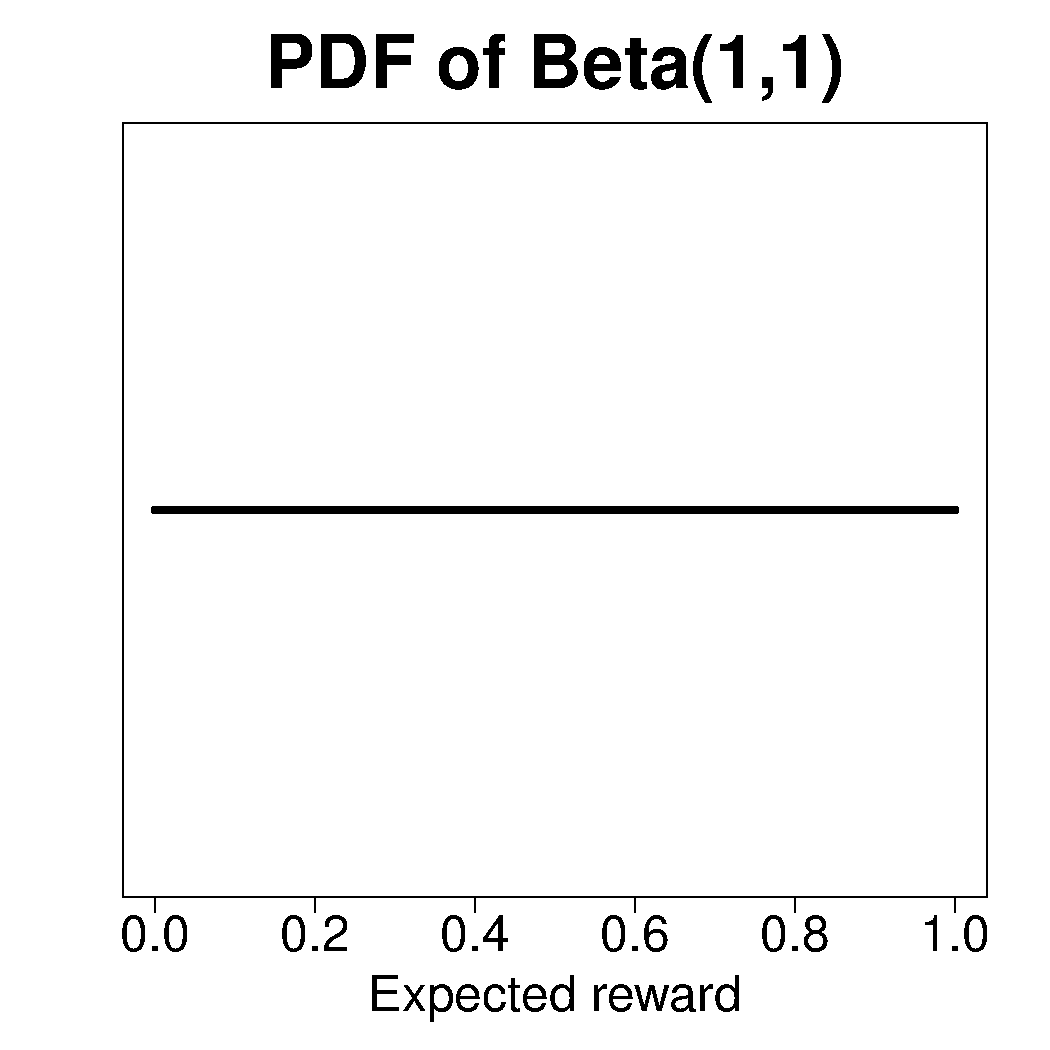
\includegraphics[width=.9\linewidth]{beta1.pdf}
    \caption{Initial situation.}
    \label{fig:beta1}
  \end{subfigure}%
  \begin{subfigure}{.30\textwidth}
    \centering
    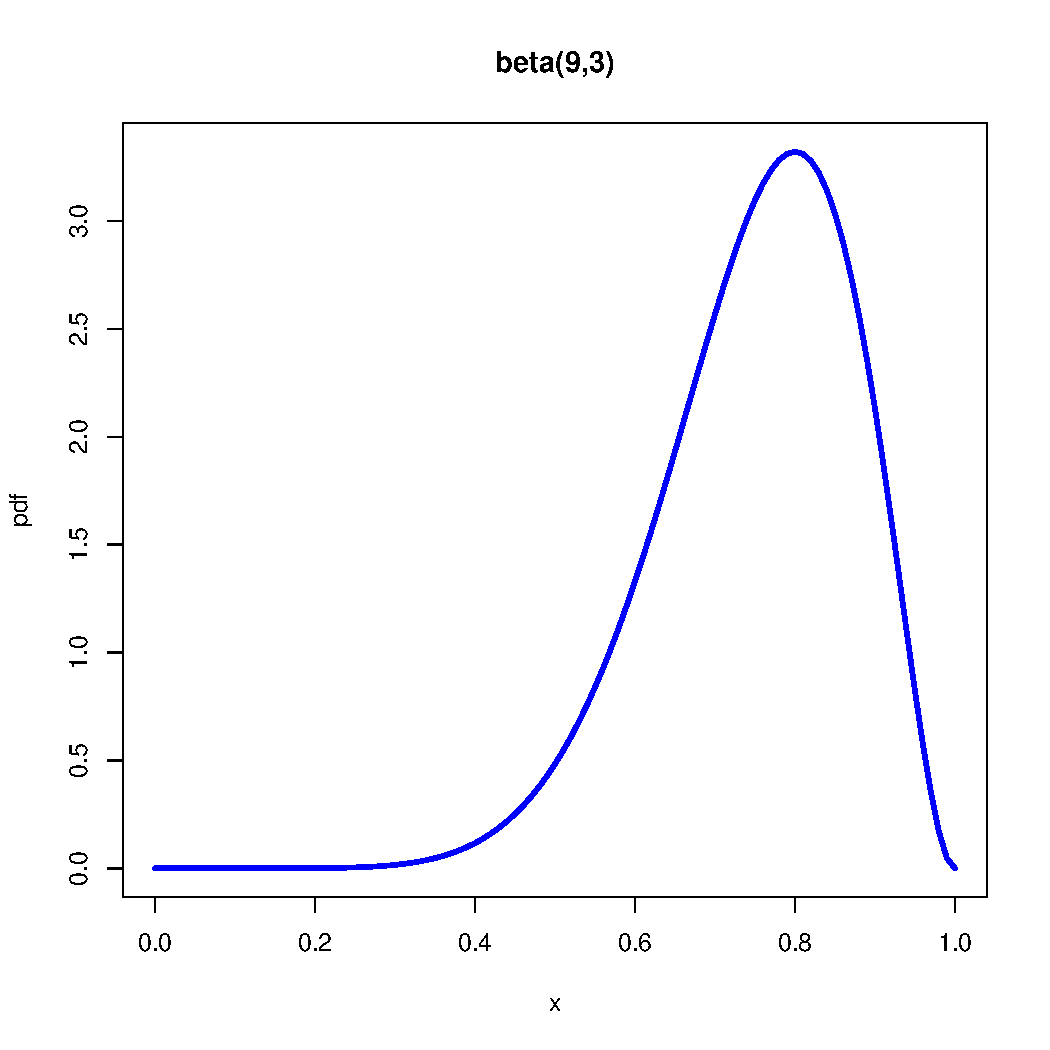
\includegraphics[width=.9\linewidth]{beta2.pdf}
    \caption{After observing many more successes than failures.}
    \label{fig:beta2}
  \end{subfigure}%
  \begin{subfigure}{.30\textwidth}
    \centering
    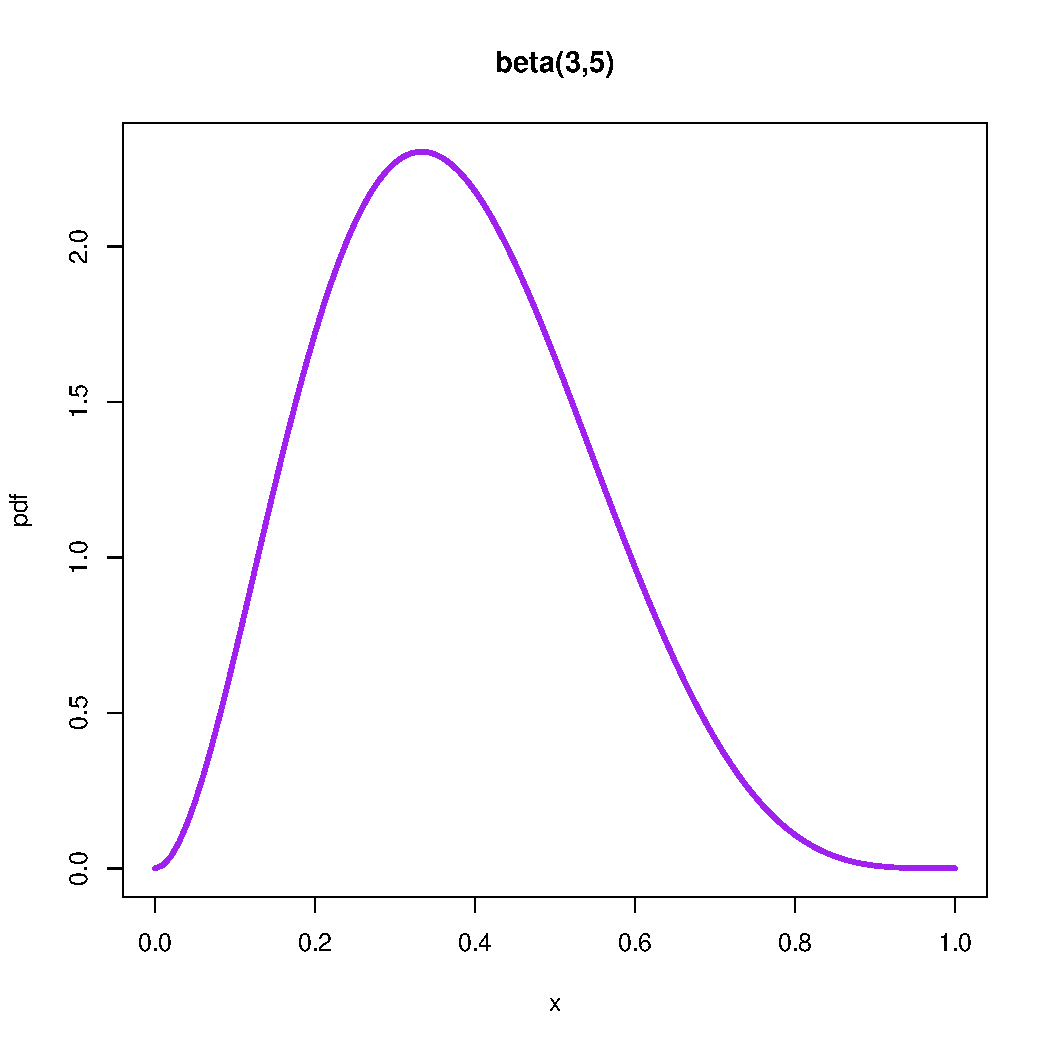
\includegraphics[width=.9\linewidth]{beta3.pdf}
    \caption{After observing slightly more failures than successes.}
    \label{fig:beta3}
  \end{subfigure}
  \caption{Illustration on what the distribution modeling the success
  probability of a Bernoulli distribution can look like.}
  \label{fig:beta}
\end{figure}



While the approach is Bayesian, it is not fully Bayesian like the Gittins
index, which although is Bayes-optimal, can't be implemented efficiently in
practice \cite{chapelle2011empirical}. The downside of Thompson sampling is
that there is a lack of theoretical analysis. Chapelle et al.
\cite{chapelle2011empirical}, however, demonstrate empirically that it
outperforms UCB and $\epsilon$-greedy methods in certain cases.
% TODO: what cases?

\subsubsection{Mortal bandits}
Most often in online advertisement, the ads (the levers) have a limited
lifespans due to limited budgets, seasonal holiday campaigns, and other
uncontrollable factors. On the other hand, new levers are introduced
occasionally in the form of new ad campaigns. This results in a stark
contradiction between reality and our model, because the multi-armed bandit
model assumes implicitly that its levers are in existence indefinitely
\cite{chakrabarti2008mortal}.

Chakrabarti et al. \cite{chakrabarti2008mortal} introduce algorithms for mortal
multi-armed bandits, a model in which levers regularly die and new ones come to
existence as replacements. One of the main results they derive is that the
regret bounds for such a situation can not be as low as for the non-mortal
case. Instead of $O(\ln t)$, a bound of $\Omega(t)$ is achieved under
mortality, $t$ being the number of rounds.

One of the main reasons for the worse bound is that in the non-mortal scenario,
after finding an optimal arm, the algorithm can thereafter concentrate on
indefinite exploitation. When arms are subjected to lifetimes, such nonchalance
is out of the question.  An especially challenging case arises when there are
many levers and short lifespans. Most likely, one must settle for suboptimality
in such a case.

The paper \cite{chakrabarti2008mortal} also describes how standard multi-armed
bandits can be adapted to take mortality into account. This is needed so that
the algorithms don't spend too much time on exploration, an investment that is
not justified under mortality. The idea of the \emph{subset heuristic} is to
divide the rounds into epochs. At the dawn of each epoch, we choose a subset
of arms uniformly at random from the set of all arms. We then run the standard
multi-armed bandit algorithm on the subset until the end of the epoch.

The classical, standard multi-armed algorithm, UCB1, is extended to allow for
mortality. Whether or not the heuristic has been applied to contextual bandits
and Thompson sampling is something the author of this seminar report couldn't
find material on. However, on the surface, there seems to be no forbidding
factors.



\subsection{Reinforcement learning}

Sometimes we may need an approach that captures more than what the $n$-armed
bandits can offer. Reinforcement learning generalizes the scenario of $n$-armed
bandits by considering a more inclusive model. We will first look at how the
full reinforcement problem can be formulated as a Markov decision process. We
will then examine some algorithms for learning optimal policies for these
processes under additional challenges brought by the banner ad domain.


\subsubsection{MDP}

A Markov decision process (MDP) \cite{book} is a 4-tuple
\begin{equation}
  (S, A, \setof{P_a : S \times S \rightarrow [0,1] \,|\, a \in A},
  \setof{R_a : S \times S \rightarrow \mathbb{R} \,|\, a \in A}).
\end{equation}

Above $S$ is a finite set of states. $A$ is a finite set of actions. Function
$P_a(s, s')$ gives the probability of transitioning to state $s'$ after
performing action $a$ in state $s$. The reward function $R_a : S \times S
\rightarrow \mathbb{R}$ gives the immediate reward obtained from performing
action $a$ in state $s$ and ending up in $s'$.

The simulation is started from an initial state $s_0$ at time 0. During each
discrete time step $t$, we are in some state $s_t$, on the basis of which we
must choose an action $a_t$, after which we are rewarded $r_t \in \mathbb{R}$,
time $t$ is incremented by one, and we end up at state $s_{t+1}$
\cite{abe2002empirical}. The task is called \emph{episodic} if there is end
state, after which the simulation is restarted. Otherwise we call the task
\emph{continuing} \cite{book}.

The central problem here, then, is to find a (near) optimal policy $\pi$ for
the agent performing the actions. Given we are in state $s_t \in S$, $\pi(s_t)$
indicates the action $a_t$ that should be performed. This can be a probability
distribution defined on set of all actions $A$. The optimal policy we wish to
find is the one that maximizes the reward accumulated over time, put formally,
maximizes $\sum_{t=0}^\infty R_{a_t}(s_t, s_{t+1})$, where $\gamma \in [0,1)$
is the discount rate.

% TODO: Prediction problem vs. Control problem

In the reinforcement learning setting, we don't know the transition
probabilities $P_a$ or the reward functions $R_a$ in advance. This entails that
in order to find an optimal policy---solve the \emph{control problem}---we
must also solve the \emph{prediction problem}, or in some sense, estimate the
transition probabilities and rewards. We do this by means of estimating a value
function.

Given a policy $\pi$, the value function $Q^\pi(s,a)$ indicates the
desirability of taking action $a$ in state $s$. The desirability is the
expected value of the cumulative reward given that we start in state $s$ and
take action $a$, after which we strictly follow policy $\pi$. The formulation
is given below, in which $r_{t+k+1}$ denotes the reward procured during time
$t+k+1$.

\begin{equation}
  Q^\pi(s,a) = E_\pi \big[ \sum_{k=0}^\infty \gamma^k r_{t+k+1} \;|\; s_t = s,
  a_t = a\big],
\end{equation}

The value function $Q^*$ of an optimal policy $\pi^*$ satisfies the
\emph{Bellman optimality equation},

\begin{equation}
  Q^*(s,a) = E\big[r_{t+1} \;|\; s_t = s, a_t = a\big]
  + \gamma E\big[\max_{a'} Q^*(s_{t+1}, a') \;|\; s_t = s, a_t = a\big]
\end{equation}

The value function $Q$ implicitly characterizes a policy. The policy
is to always choose the action that maximizes the value function, or, $\pi(s) =
\arg\max_a Q(s,a)$. In the case of optimal value function $Q^*$, following this
method leads to the optimal policy $\pi^*$ \cite{abe2002empirical}.

%TODO: value function

The standard multi-armed bandit can be viewed as a Markov decision process in
which there is exactly one state. The levers of the bandit are all the possible
actions, and performing an action always brings you back to the initial state.
The contextual bandit model does have different states, but the action chosen
doesn't impact the choice of the next state.


\subsubsection{Direct, indirect and semi-direct reinforcement learning}

\subsubsection{Concurrent reinforcement learning}

\begin{itemize}
  \item{Motivate need for concurrent reinforcement learning in targeted
    advertising.}
  \item{Introduce TD($\lambda$)-learning algorithms.}
  \item{Introduce concurrent reinforcement learning.}
\end{itemize}


\subsection{Function approximation}
Almost all the implementations \cite{abe2002empirical, silver2013concurrent,
chapelle2011empirical} of targeted advertising considered in this seminar
report required some sort of function approximation, regardless of whether they
were bandit or reinforcement based.

In real world (advertisement) data there tends to be a huge amount of features,
which means that if we treat the state space of the reinforcement learning
problem as the feature space, we get a huge explosion in the number of states
\cite{abe2002empirical}.  This means that most likely the reinforcement
learning will not know to behave desirably in never-before-seen states
\cite{book}.

TODO:
\begin{itemize}
  \item{Define function approximation precisely: "We estimate and represent the
    value function as a function of state features and actions"}
  \item{Relation to supervised machine learning.}
  \item{In my examples: multivariate linear regression}
\end{itemize}


\section{Conclusions}

\subsubsection*{References}
\nocite{*}

\printbibliography[heading=none]


\end{document}
